\chapter{The Elicited Imitation Task}\label{sec:3}

\section{Research questions and hypotheses}\label{sec:04:1}

While a more detailed discussion of the theoretical premises of the Elicited Imitation test (EIT) was given in \chapref{sec:1}, it is worthwhile to repeat here that according to its rationale, the task does not require learners to simply repeat a string of sounds, but rather to decode its meaning and re-produce it ``in their own words'', i.e. based on the present state of their interlanguage grammar. In this respect, the task is used in this work as an approximation of a productive task. Unlike in free production tasks, however, EI makes it possible to maintain full control over the target structure, which seems particularly urgent in the case of rare, non-obligatory targets such as the OS structures investigated in this work.

The present chapter describes the structure of the VILLA EI task and presents the results obtained by the various L1 groups of the project. The analysis aims to identify the impact that independent variable: word order in target sentence, input, and L1 exert on dependent variable: accurate repetition of inflectional markers. Based on the information presented in the introduction, the following hypotheses may be formulated regarding the effect of the variables taken into consideration.

\begin{itemize}
    \item Word order: SO targets are expected to be processed with greater ease than the corresponding OS targets. This is due to the greater frequency of SO structures in the VILLA input as well as to their general unmarkedness from a pragmatic and typological point of view.
    \item L1: source languages in which case is expressed morphologically (such as German) should prove an advantage in the processing of a highly inflected L2 like Polish. Conversely, the rigid word order and lack of inflectional morphology of English and (spoken) French may slow down the acquisition process.
    \item Exposure to the input: greater length of exposure to the input (measured in hours) is expected to be beneficial to the development of the learners’ morphosyntactic skills.
\end{itemize}

Finally, an attempt will be made to correlate the results of the EI task with the Llama D test of implicit influence of pattern recognition ability on phonological memory, in order to verify whether or not the learners’ repetition performance is influence by this variable, whose involvement is typically excluded in the description of the rationale of the EI task.

\section{Results}\label{sec:04:2}

\subsection{Overview of learner output: overall repetition accuracy}\label{sec:04:2.1}

Overall repetition accuracy refers to the number of target segments which are correctly reproduced in a learner’s response. For the time being, the analysis will exclude inflectional endings, which will be treated in greater detail in the next sections. From a strictly phonological point of view, case endings such as [a] and [e] are segments like any other in the target string, and could therefore contribute to a measure of phonological accuracy. On the other hand, in the target language they are also inflectional morphemes conveying grammatical information. According to the assumptions of the EI task, the learner \textit{might} use them to derive and express syntactic functions, if the interlanguage has developed a morphosyntactic principle of utterance organisation: however, there are no \textit{a priori} means to establish whether that is the case or not. In short, it is hard to tell if the distribution of case endings is due to reasons pertaining to phonology (because the learner heard them that way) or morphosyntax (because the learner wanted to express a given syntactic function using the corresponding case ending).

Turning to an overview of phonological accuracy, most of the times lexical items appear to be fairly recognisable. Linguistic material may be omitted \REF{ex:04:1} or substituted \REF{ex:04:2}: compare the target in a. with learner output in b. 

\ea%1
    \label{ex:04:1}
    \ea\label{ex:04:1a}
    /ʤef'ʧink 'ʧongnie portu'galk/
    \ex\label{ex:04:1b}
    [ʤef'ʧink ʧon portu'galk]
    \z
\z

\ea%2
    \label{ex:04:2}
    \ea\label{ex:04:2a}
    /ʤef'ʧink 'ʧongnie portu'galk/
    \ex\label{ex:04:2b}
    [dy'ʧink 'bardzo portu'galk]
    \z
\z

In extreme cases, words may be mispronounced so badly that it is no longer possible to map them to existing word forms of the input, as [ʧyʒank] in \REF{ex:04:3}. At times, learner output appears to combine bits of two or more words from the input, as in \REF{ex:04:4}\footnote{See \citet{Saturno2015} for a discussion of similar examples and of the implications of transcription for all subsequent stages of data analysis.}, in which the item [unʧe'ʧelk] shows traces of the input words \textit{dziewczyna} [ʥefˈʧɨna] ‘girl’ and \textit{nauczycielka} [nauʧɨˈʨelka] ‘teacher’.

\ea%3
    \label{ex:04:3}
    /studentke pxa nauʧiʧelka/\\{}
    [ʧy'ʒank 'pxa unʧe'ʧelk]
    \z

\ea%4
    \label{ex:04:4}
    /portu'galk 'ʧongnie ʤefʧink/\\{}
    [portu'galk 'ʧoni ʧef'ʧelk]
    \z

\subsection{Overview of learner output: repetition of case endings}\label{sec:04:2.2}

The following transcripts present examples of correct \REF{ex:04:6} and incorrect \REF{ex:04:7} repetition of the case ending -[e] in identical target sentences, reported in \REF{ex:04:5}. Each sentence is followed by the speaker’s code and the time it was uttered. In incorrect repetitions both nouns are marked as -[a], on the model of the nominative case in the input, whereas in target-like output the two nouns are marked with different endings. Typically, each sentence presents either one or no errors.

\ea%5
    \label{ex:04:5}
    \ea\label{ex:04:5a}
    \gll    /artɨstk-e   pozdravja   twumatʃk-a/\\
            artist-\textsc{acc}  cheers    interpreter-\textsc{nom}\\
    \glt    ‘The interpreter cheers the artist.’
    \ex\label{ex:04:5b}
    \gll    /ʥevtʃɨŋk-a  ʨɔŋgnje   portugalk-e/\\
            little.girl-\textsc{nom}  pulls    Portuguese.woman-\textsc{acc}\\
    \glt    ‘The little girl pulls the Portuguese woman.’
    \ex\label{ex:04:5c}
    \gll    /brazɨlijk-a     vɔwa   kuxark-e/\\
            Brazilian.woman-\textsc{nom}  calls  cook-\textsc{acc}\\
    \glt    ‘The Brazilian woman calls the cook.’
    \z
\z

\ea%6
    \label{ex:04:6}
    \ea{\label{ex:04:6a}
    \gll    [artist-e  pɔzdravja   tumatʃk-a]\\
            artist-\textsc{acc}  cheers    interpreter-\textsc{nom}\\}\jambox*{(5104, T2)}
    \ex{\label{ex:04:6b}
    \gll    [dʒevtʃjenk-a  dʒɔnkje  portugalk-e]\\
            little.girl-\textsc{nom}  pulls    Portuguese.woman-\textsc{acc}\\}\jambox*{(5118, T1)}
    \ex{\label{ex:04:6c}
    \gll    [brazilik-a     vo'a   kurark-e]\\
            Brazilian.woman-\textsc{nom}  calls  cook-\textsc{acc}\\}\jambox*{(1119, T2)}
    \z
\z


\ea%7
    \label{ex:04:7}
    \ea{\label{ex:04:7a}
    \gll    [artistk-a   posdravja   tumatʃk-a]\\
            artist-\textsc{nom}  cheers    interpreter-\textsc{nom}\\}\jambox*{(2117, T2)}
    \ex{\label{ex:04:7b}
    \gll    [dʒevtʃinkn-a hm hm   portugalk-a]\\
            little.girl-\textsc{nom}  omission  Portuguese woman-\textsc{nom} \\}\jambox*{(4122, T1)}
    \ex{\label{ex:04:7c}
    \gll    [brazilik-a     wave   kukark-a]\\
            Brazilian woman-\textsc{nom}  calls  cook-\textsc{nom}\\}\jambox*{(3118, T1)}
    \z
\z

The same may happen with the repetition of -[a] NOM, although this is a much rarer event. The substitution of target -[a] with the competing ending -[e] produces a sentence in which both nouns are marked as -[e] (\REF{ex:04:8a}; target in \REF{ex:04:8b}).
\ea%8
    \label{ex:04:8}
    \ea{\label{ex:04:8a}
    \gll    [brazilijk-ɛ     vowa   vowa   kuxark-ɛ]\\
            Brazilian.woman-\textsc{acc}   calls   calls   cook-\textsc{acc}\\}\jambox*{(4113, T1)}
    \ex\label{ex:04:8b}
    \gll    /brazɨlijk-e     vɔwa     {} kuxark-a/\\
            Brazilian.woman-\textsc{acc}   calls     cook-\textsc{nom}\\
    \glt    ‘The cooks calls the Brazilian woman.’
    \z
\z
In rare instances, sentence with two errors may occur, in which case endings are swapped (\REF{ex:04:9a}; target in \REF{ex:04:9b}). 

\ea%9
    \label{ex:04:9}
    \ea{\label{ex:04:9a}
    \gll    [brazilijk-a     vowa   kuxark-e]\\
            Brazilian.woman-\textsc{nom}   calls   cook-\textsc{acc}\\}\jambox*{(2104, T1)}
    \glt    
    \ex\label{ex:04:9b}
    \gll    /brazɨlijk-e     vɔwa   kuxark-a/\\
            Brazilian.woman-\textsc{acc}   calls   cook-\textsc{nom}\\
    \glt    ‘The cook calls the Brazilian woman.’
    \z
\z

\subsection{Repetition of –[e]}\label{sec:04:2.3}

\subsubsection{Descriptive statistics}\label{sec:04:2.3.1}

The EI task was scored as follows: for each combination of time, word order and target ending, the scores of one or zero were assigned depending on whether or not the learner-produced output matched the expected target. The sum of these score was then divided by the number of targets produced (typically eight, but possibly less as a result of omissions or unrecognisable output, which were excluded from the analysis).

SO targets are generally processed with greater accuracy than OS ones, although scores remain rather low - below 50\% in most cases. Mean scores vary greatly across L1s, suggesting that there may be an important influence of the native language. Finally, variance is very high, which indicates that learners perform very differently from each other.

Information as to the performance of individual learners at T1 is presented graphically in \figref{fig:04:1}. In addition to standard boxplots, the individual data points are presented; their size is directly proportional to the number of learners achieving each score (also specified by the digits in white). Descriptive group statistics are provided in \tabref{tab:04:1}.

\begin{figure}
    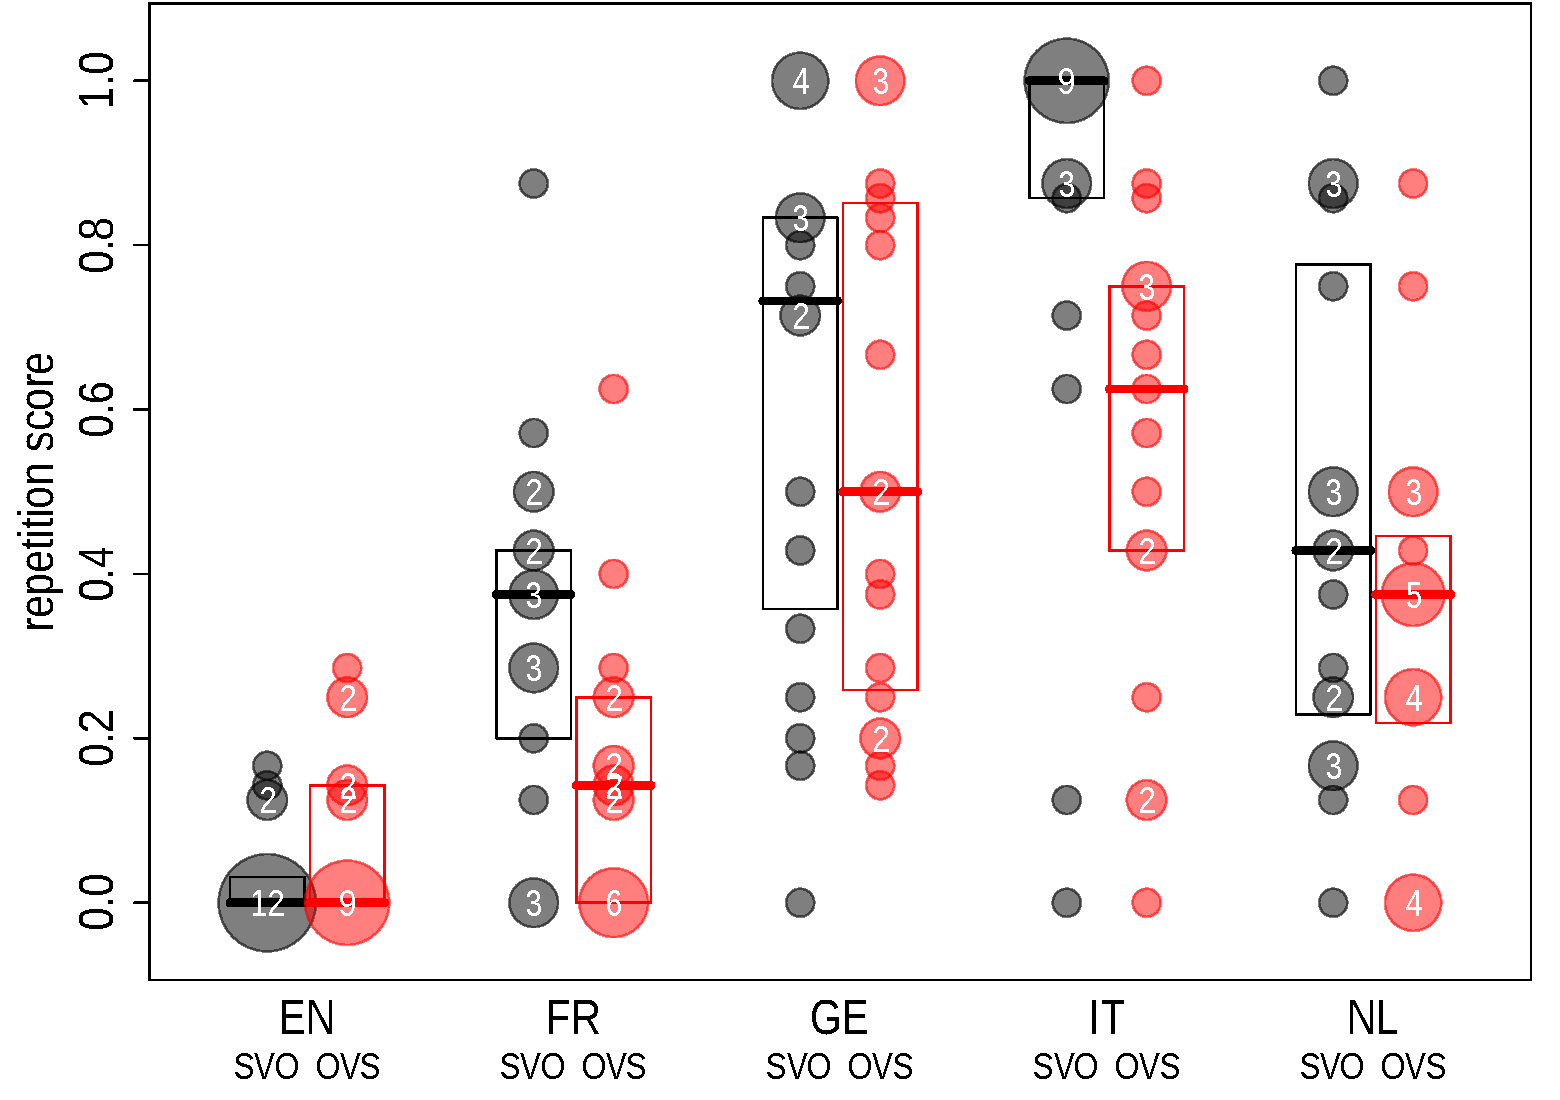
\includegraphics[width=\textwidth]{figures/04-1.pdf}
    \caption{EI task, [e] targets, T1, scores by L1}
    \label{fig:04:1}
\end{figure}

\begin{table}
    \begin{tabularx}{\textwidth}{XXXXXXX}
    \lsptoprule
    L1 & \multicolumn{3}{c}{ SO} & \multicolumn{3}{c}{ OS}\\
    & mean & sd & n & mean & sd & n\\
    \cmidrule{2-7}
    FR & 0.34 & 0.48 & 123 & 0.16 & 0.37 & 119\\
    GE & 0.62 & 0.49 & 82 & 0.57 & 0.50 & 110\\
    IT & 0.83 & 0.37 & 126 & 0.55 & 0.50 & 129\\
    NL & 0.48 & 0.50 & 147 & 0.33 & 0.47 & 155\\
    EN & 0.04 & 0.19 & 108 & 0.09 & 0.29 & 112\\
    \lspbottomrule
    \end{tabularx}
    \caption{EI task L1 descriptive statistics, -[e] ending, SO targets, T1}
    \label{tab:04:1}
    \label{tab:03:1}
\end{table}

The English L1 group consistently exhibits the poorest results, with most learners scoring exactly 0\%. No learner in this group ever scored over about 30\%. In contrast, the Italian group has the highest scores, followed by the German group and by the Dutch and French, somewhat behind. In all groups except the English and the French, at least one learner managed to reach 100\% accuracy. 

Individual variability within the L1 groups is extremely high, with learners’ scores ranging from 0\% to 100\%. The only exception, again, is the English group, in which scores are consistently close to floor level.

The picture looks fairly similar at T2 (\figref{fig:04:2} and \tabref{tab:04:2}), although a general improvement can be observed in the data.

\begin{figure}
    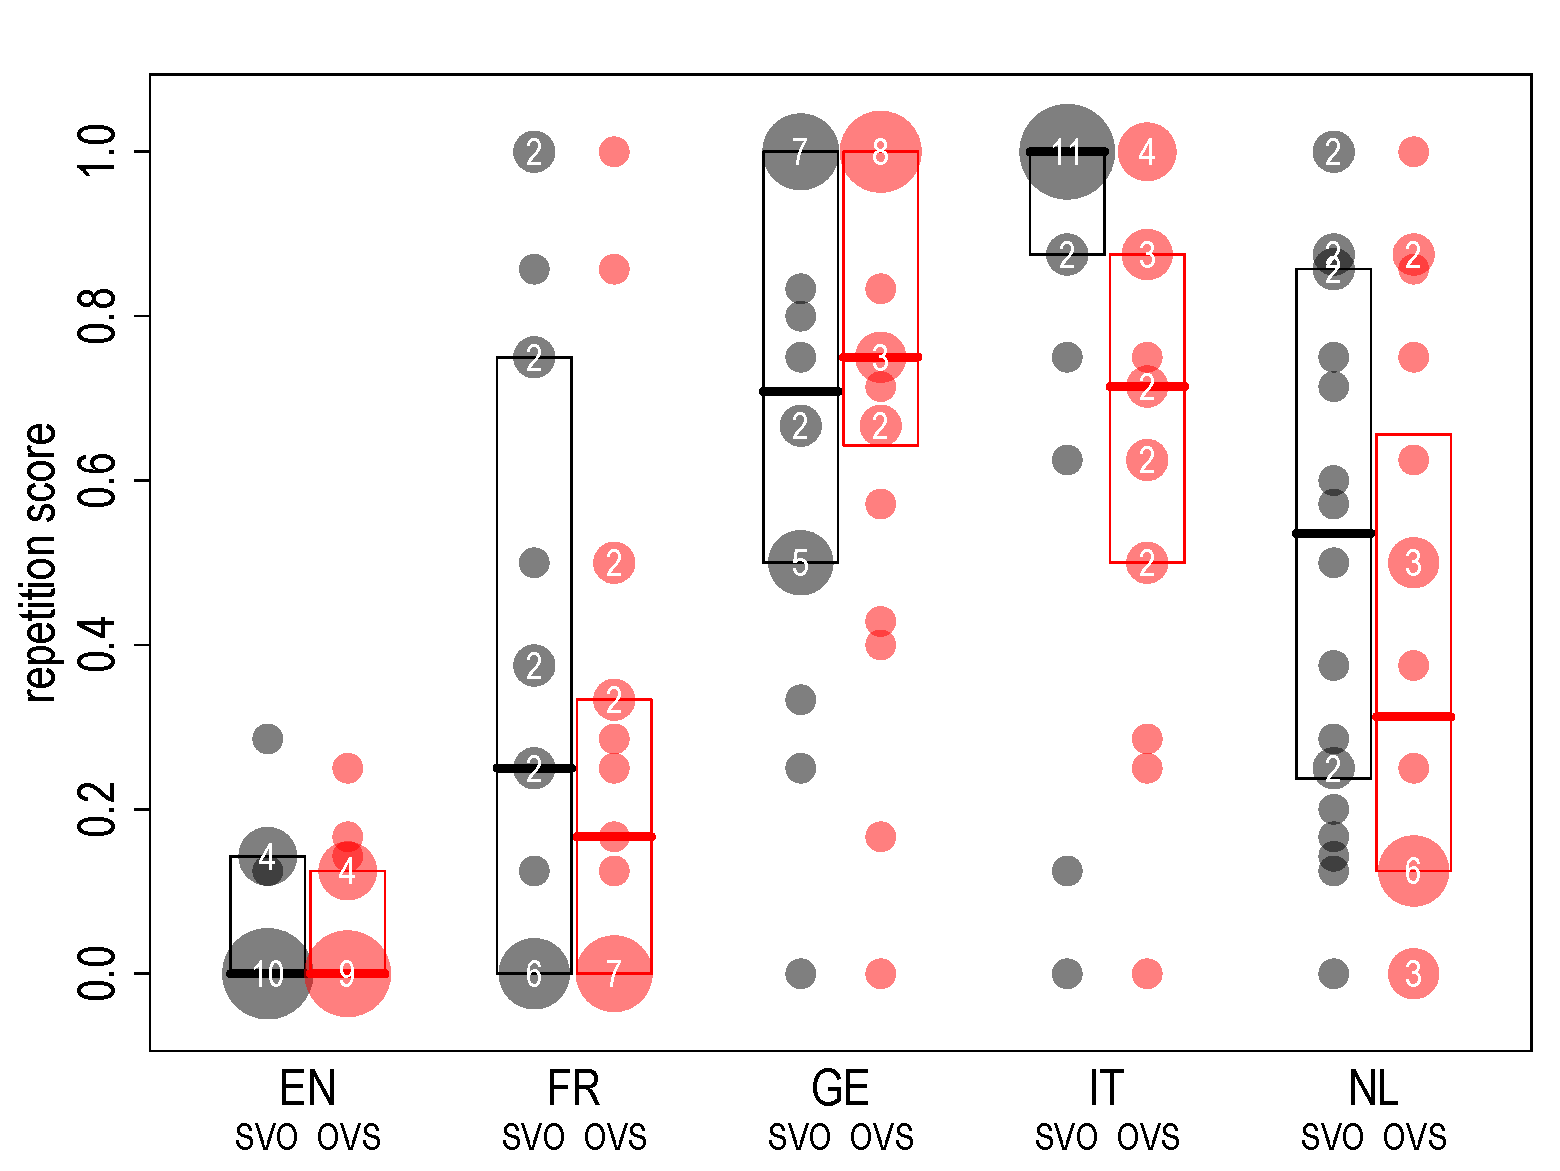
\includegraphics[width=\textwidth]{figures/04-2.pdf}
    \caption{EI task, [e] targets, T2, scores by L1}
    \label{fig:04:2}
\end{figure}

\begin{table}
    \begin{tabular}{lrrr rrr}
    \lsptoprule
    L1 & \multicolumn{3}{c}{ SO} & \multicolumn{3}{c}{ OS}\\
    & mean & sd & n & mean & sd & n\\
    \cmidrule(r){2-4}\cmidrule(l){5-7}
    FR & 0.39 & 0.49 & 126 & 0.26 & 0.44 & 121\\
    GE & 0.69 & 0.46 & 72 & 0.74 & 0.44 & 111\\
    IT & 0.87 & 0.34 & 127 & 0.69 & 0.47 & 131\\
    NL & 0.53 & 0.50 & 146 & 0.39 & 0.49 & 157\\
    EN & 0.06 & 0.24 & 118 & 0.07 & 0.25 & 118\\
    \lspbottomrule
    \end{tabular}
    \caption{EI task descriptive statistics, -[e] ending, OS targets}
    \label{tab:04:2}
    \label{tab:03:2}
\end{table}

\subsubsection{Inferential statistics}\label{sec:04:2.3.2}

A generalised linear mixed model \citep{Baayen2008} with binomial error structure and logit link function (Likelihood Type 3-test) was fitted to the data. Fixed effects comprised the L1 (five levels, reference level = EN), word order (binary, reference level = OS) and time (binary, reference level = T1) and the Llama test score (continuous, 0 to 1) as linear predictors, as well as the following two-way interactions: L1:word order, L1:time, and time:word order. Random effects included random intercepts for target sentence and participants as well as within-subject uncorrelated random slopes for time and word order. 

The rationale for including the interactions was as follows. The learners' ability to correctly repeat -[e] may be influenced by the word order of the target sentence, with SO targets generally facilitating correct repetition, and OS targets hindering it. In turn, the extent of this word order effect may be variably influenced by the learner’s L1. Further exposure is thought to be generally beneficial to repetition, but the extent to which results improve between T1 and T2 may be also determined by the learners’ L1: speakers of certain languages may improve more markedly than speakers of other languages. The effect of time is also likely to be constrained by word order. 

The summary of the model is presented in \tabref{tab:04:3}.

\begin{table}
    \begin{tabularx}{\textwidth}{Xrrr}
    \lsptoprule
    \textbf{~} & \multicolumn{3}{c}{ \textbf{response}}\\
    \textit{Predictors} & \textit{Odds} \textit{Ratios} & \textit{CI} & \textit{p}\\
    \midrule
    (Intercept) & 0.02 & 0.01~–~0.10 & \textbf{<0.001}\\
    time [2] & 0.76 & 0.22~–~2.62 & 0.661\\
    L1 [FR] & 2.79 & 0.85~–~9.19 & 0.091\\
    L1 [GE] & 38.27 & 11.65~–~125.66 & \textbf{<0.001}\\
    L1 [IT] & 15.27 & 3.96~–~58.84 & \textbf{<0.001}\\
    L1 [NL] & 9.70 & 3.01~–~31.24 & \textbf{<0.001}\\
    WO2 [SO] & 0.45 & 0.12~–~1.64 & 0.225\\
    llama & 4.57 & 0.71~–~29.39 & 0.110\\
    time [2] * L1 [FR] & 1.71 & 0.37~–~7.88 & 0.491\\
    time [2] * L1 [GE] & 2.97 & 0.65~–~13.68 & 0.161\\
    time [2] * L1 [IT] & 3.31 & 0.70~–~15.75 & 0.132\\
    time [2] * L1 [NL] & 1.96 & 0.46~–~8.38 & 0.362\\
    time [2] * WO2 [SO] & 0.93 & 0.57~–~1.53 & 0.775\\
    L1 [FR] * WO2 [SO] & 6.17 & 2.22~–~17.19 & \textbf{<0.001}\\
    L1 [GE] * WO2 [SO] & 3.13 & 1.06~–~9.30 & \textbf{0.040}\\
    L1 [IT] * WO2 [SO] & 19.50 & 6.26~–~60.74 & \textbf{<0.001}\\
    L1 [NL] * WO2 [SO] & 5.17 & 1.95~–~13.74 & \textbf{0.001}\\
    \multicolumn{4}{c}{\textbf{Random} \textbf{Effects}}\\
    σ\textsuperscript{2} & \multicolumn{3}{c}{3.29}\\
    τ\textsubscript{00}~\textsubscript{participant} & \multicolumn{3}{c}{1.41}\\
    τ\textsubscript{00}~\textsubscript{target\_no} & \multicolumn{3}{c}{0.87}\\
    τ\textsubscript{11}~\textsubscript{participant.WO2SO} & \multicolumn{3}{c}{2.19}\\
    τ\textsubscript{11}~\textsubscript{participant.time2} & \multicolumn{3}{c}{2.37}\\
    ρ\textsubscript{01}~\textsubscript{participant.WO2SO} & \multicolumn{3}{c}{1.00}\\
    ρ\textsubscript{01}~\textsubscript{participant.time2} & \multicolumn{3}{c}{{}-0.14}\\
    N~\textsubscript{participant} & \multicolumn{3}{c}{90}\\
    N~\textsubscript{target\_no} & \multicolumn{3}{c}{16}\\
    \midrule
    Observations & \multicolumn{3}{c}{2438}\\
    Marginal R\textsuperscript{2}~/ Conditional R\textsuperscript{2} & \multicolumn{3}{c}{0.550 / NA}\\
    \lspbottomrule
    \end{tabularx}
    \caption{Model summary}
    \label{tab:04:3}
\end{table}

The Llama score does not appear to be a significant predictor, which suggests that sensitivity to phonological patterns is not involved in determining success at the EIT. The three hypothesised interactions were explored by comparing the full model described above to three null models, each lacking the single interaction of interest. Statistical significance was assessed based on likelihood ratio tests: P values were corrected for multiple comparison using the Holm correction. The results are presented in \tabref{tab:04:4}.

\begin{table}
    \begin{tabularx}{.8\textwidth}{Xrrr}
    \lsptoprule
    predictor & Chisq & Chi Df & p\\
    \midrule
    time :L1 & 3.023 & 4 & > 0.05\\
    time : word order & 0.812 & 1 & > 0.05\\
    L1 : word order & 32.607 & 4 & < 0.01\\
    \lspbottomrule
    \end{tabularx}
    \caption{Full/null model comparisons}
    \label{tab:04:4}
\end{table}

Only the interaction involving L1 and word order proved to be statistically significant, which indicates that the impact of word order (SO vs. OS) varies based on the learner’s L1. 

The significant interaction was subsequently explored through pairwise comparison. The results relative to the role of the L1 are presented in \figref{fig:04:3}, in which blue bars represent confidence intervals for least square means. Pairwise comparisons are statistically significant if the red arrows do not overlap. Statistically significant contrasts are presented in \tabref{tab:04:5}.

\begin{table}
    \begin{tabularx}{\textwidth}{lQ}
    \lsptoprule
    Condition & pairwise comparison\\
    \midrule
    T1 OS & EN < GE (p < 0.01), IT (p <.01), NL (p < 0.01);\newline
    FR < GE (p <0 .01), IT (p < 0.01)\newline
    NL < GE (p = 0.04)\\
    \tablevspace
    T1 SO & EN < FR (p < 0.01), GE (p < 0.01), IT (p <.01), NL (p < 0.01)\newline
    FR < GE (p = 0 .01), IT (p < 0.01)\\
    \tablevspace
    T2 OS & EN < GE (p < 0.01), IT (p <.01), NL (p < 0.01);\newline
    FR < GE (p <0 .01), IT (p < 0.04)\\
    \tablevspace
    T2 SO & EN < FR (p < 0.01), GE (p < 0.01), IT (p <.01), NL (p < 0.01)\newline
    FR < GE (p < 0 .01), IT (p < 0.01)\\
    \lspbottomrule
    \end{tabularx}
    \caption{Pairwise comparisons, L1 : word order interaction (only significant contrasts shown)}
    \label{tab:04:5}
\end{table}

\begin{figure}
    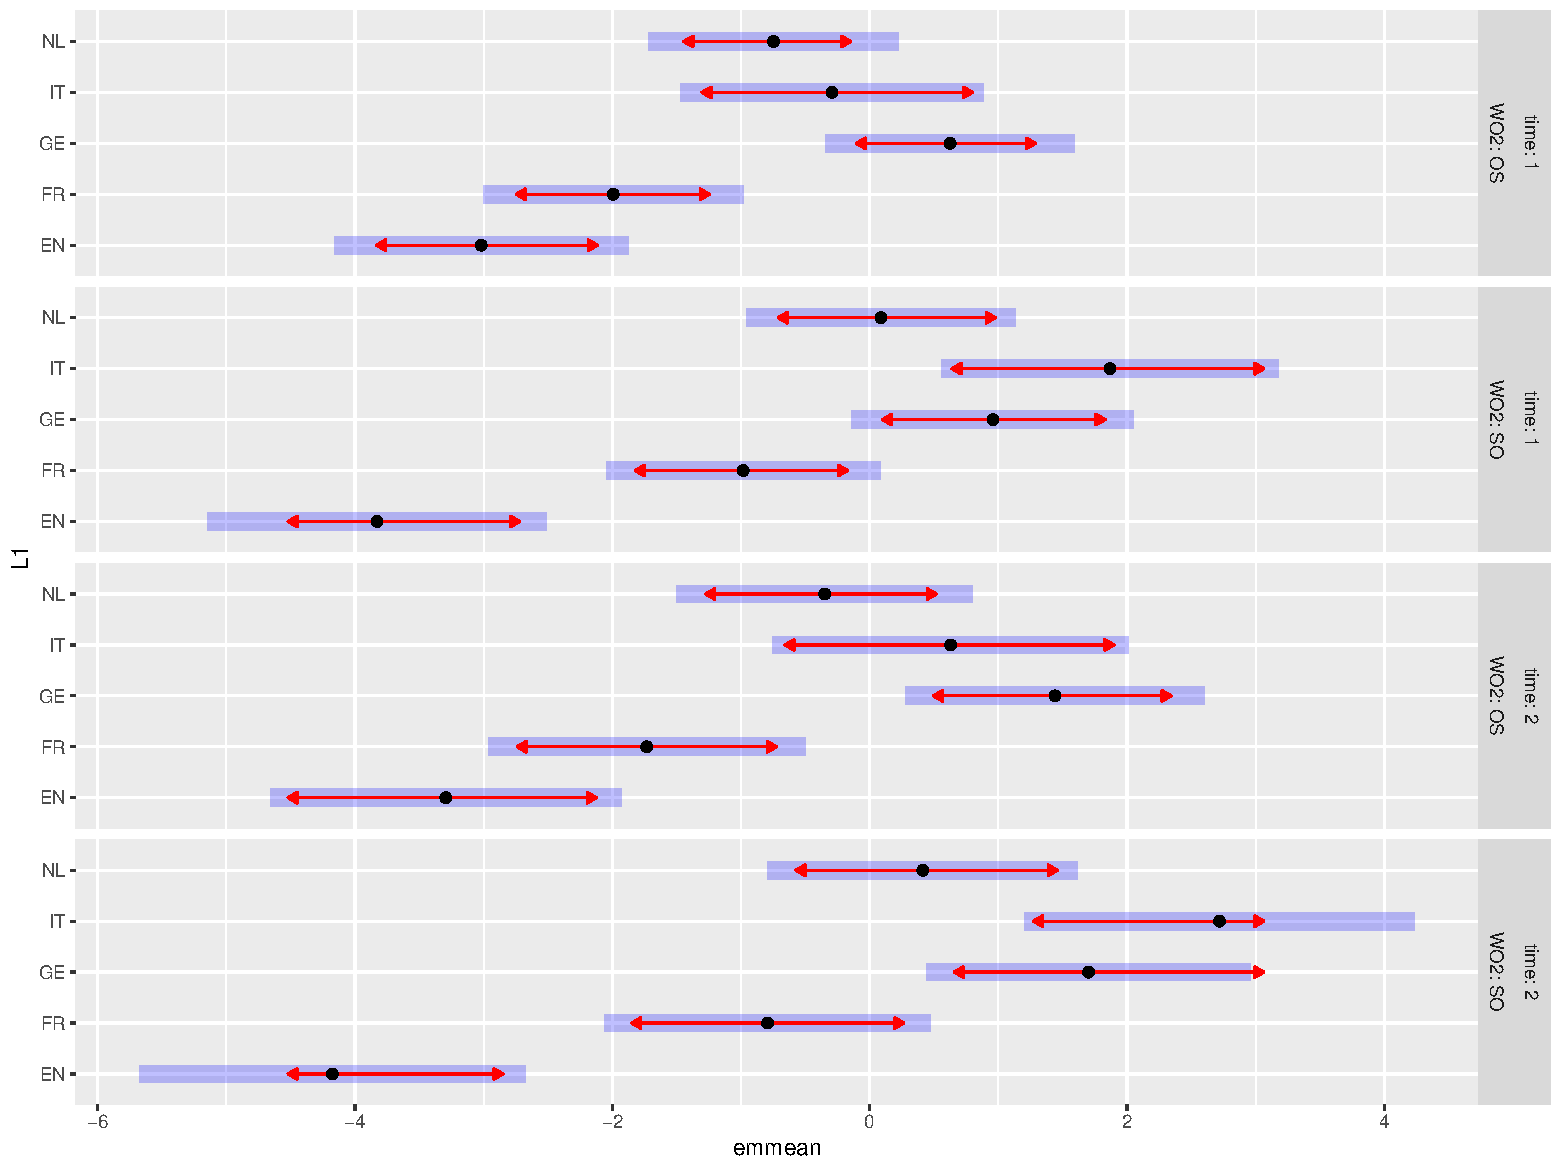
\includegraphics[width=\textwidth]{figures/04-3.pdf}
    \caption{Pairwise comparisons, L1 : word order interaction}
    \label{fig:04:3}
\end{figure}

Turning to the effect of word order (\figref{fig:04:4}), it appears that although SO targets generally produce higher scores (except for the L1 English group), the difference is only significant for the L1 Italian group (p < 0.01 at both test times).

\begin{figure}
    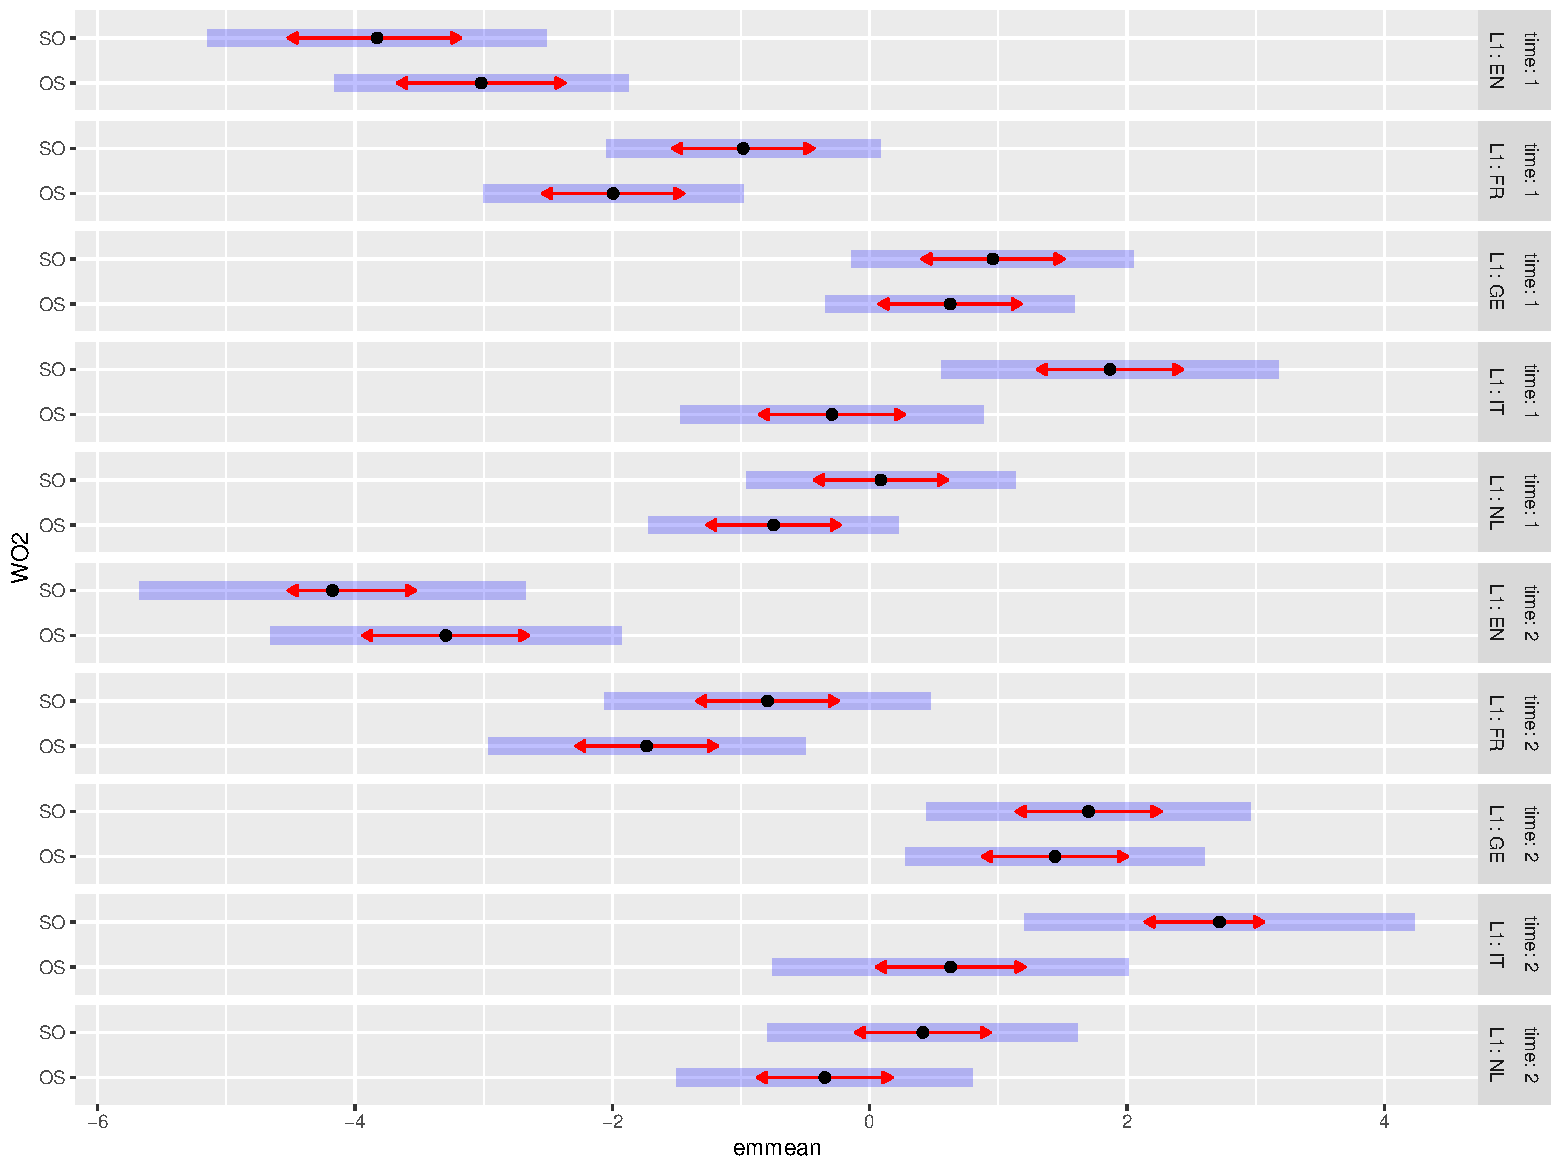
\includegraphics[width=\textwidth]{figures/04-4.pdf}
    \caption{Pairwise comparisons, word order: L1 interaction}
    \label{fig:04:4}
\end{figure}

\subsection{A different perspective}\label{sec:04:2.4}

The analysis presented thus far has shown that certain L1s seem to be associated to higher repetition accuracy when compared to other languages: for instance, French speakers scored on average 0.16 at T1 on the repetition of -[e], whereas the Italians scored 0.55. From this one might conclude that L1 Italian has a positive effect on processing accuracy. These, however, are but mean values, collapsing the results of an entire group. But individual learner performance may vary greatly even within the same L1 group, making the idea of a ``group interlanguage'' quite problematic. Thus, alongside group averages, which may be informative as to the role of a given L1 on the average groups scores, it seems worthwhile to describe learners in terms of their individual processing strategies, operationalised as a set of scenarios. Such outcome would be particularly welcome for an analysis rooted on the Learner Variety theoretical paradigm. Therefore, individual profiling will be used throughout the book to present an alternative view to inferential statistics: it is argued that combined, the two methods may contribute to a better description and interpretation of the data. The present section describes the rationale of this approach.

Within this study, processing profiles may be seen as belonging to three scenarios: 

\begin{itemize}
    \item[a)] learners rely on a single uninflected word-form of each lexical item, with no morphological variation;
    \item[b)] learners may have \textit{noticed} some morphological variation in the input, but they cannot make sense of it based on a systematic rule. Therefore, these learners will supply the basic and inflected word-forms with no apparent regularity;
    \item[c)] learners regularly produce correctly inflected word-forms.
\end{itemize}

Scenario b) might be called chance performance, roughly equivalent to guessing. With only two values to choose from (-[a] and -[e]), accuracy rates should be around 50\%. Scenario a) is \textit{below} chance: learners who behave in this way are not guessing, but applying a systematic principle, which, alas, is not compatible with the target language and thus produces accuracy rates tending to 0\%. Specifically, this principle maintains that all feminine nouns, independently of their syntactic function, are characterised by word-final -[a]. Syntactic functions are expressed by the position of a noun in the utterance.

Finally, scenario c) is \textit{above} chance: learners systematically apply a principle of case marking which is apparently coherent with the regularities of the target language, although in an EI test the possibility cannot be ruled out that target-like performance in fact derives from particularly developed phonological memory.

In order to assign learners to the corresponding scenarios, one needs to statistically compute the probability of observing a given result on the basis of a statistical distribution which appropriately models the task at hand. The binominal distribution describes the probability of obtaining either of two values (conventionally 0 and 1) out of a given number of trials, as in the throwing of a coin. Statistical tests based on this distribution make it possible to answer such questions as ``what is the probability of obtaining head six times if one throws a coin eight times?''. If the probability is too small, conventionally below 5\%, one may conclude that the coin is not fair, i.e. that it is biased towards a particular result. In the present experiment, the same question would sound as follows: ``what is the probability that a learner, without applying a morphosyntactic principle, produced six instances of correct case-marking over eight trials?'' Again, if the probability is too small, one should conclude that performance is not random, i.e. that the learner is applying a morphosyntactic principle.

The modelling of the EI task as a coin throwing experiment may seem questionable on several grounds. Indeed, such an approximation is fairly intuitive in the context of a forced-choice response task, such as the Comprehension task described in Chapter 5, in which learners are simply asked to select the correct alternative out of two possible responses. If they pay no attention at all to the target sentence, and only chose pictures through guessing, then the probability that either picture is selected should be 50\%. This is not the case in the EI task, in which participants are required to actively produce output, the model for which (i.e., the expected response) is provided in the stimulus sentence. 

Moreover, the two possible answers [a] and [e] may not be equally probable or available to the learner. In fact, as it will be shown in \chapref{sec:8}, [a] seems to be the unmarked, basic word-form of lexical items, so that if either ending tends to overextend onto the other, most probably it will be [a] overextending onto [e]. More generally, it is common for initial learner varieties to overextend any given word-form onto all others: clearly, the overextended value should be seen as more probable. In the present context, repeating [e] should require a conscious effort on the side of the learner, thus mirroring an intentional strategy.

Finally, the guessing of a binary value relies on the assumption that the trial may only result in two values. This is indeed the rationale of the VILLA EI test, in which the target structure only opposes [a] to [e]. However, it is impossible to tell whether or not learners were aware that the task only targeted two inflectional endings, especially if one considers that it also included a variety of other structures as distractors: learner output thus may be potentially more varied than that, as even in the limited VILLA input lexical items occur in more than just two word-forms. In sum, the possibility that learners performed the task by guessing alone might seem rather remote.

While this all is true, in principle, the reality is slightly different. The unmarkedness of [a] certainly contributes to explaining why [e] repetition scores tend to zero in some learners, who consistently produced the alternative ending in all contexts. Intermediate scores, however, fit into this picture less well and suggest that target items do imply a choice between [a] and [e], at least in some learners. Regarding the argument that if learners were guessing, then they would produce more than just two endings, it appears that the cases in which learners produce an ending other than -[a] or -[e] (with the exclusion of centralised -/ə/) are extremely rare. After all, the EI task does include a stimulus question in which the expected response is provided. If participants listen carefully to these sentences (which is obviously a prerequisite for the successful completion of the task), they may notice that a) target nouns exhibit some variation across target sentences, and b) that variation only contrasts [a] to [e]. Thus, it does not seem unlikely that the set of possible endings in the learner’s mind only comprises [a] and [e], even though other forms occur in the input. Nevertheless, this does not imply that the learner has already identified the regularity which governs their distribution in the input. If that is the case, then the learner might know that either [a] or [e] is required in the task, but will not be able to tell which should be supplied in the individual target sentences: under these circumstances, randomly supplying either ending, i.e. guessing, may indeed sound like a realistic strategy.

To summarise, one should first ask whether or not the individual learner noticed that target nouns vary in their inflectional ending, the possible options being [a] and [e]. If not, the learner will consistently apply a positional principle, so that the statistical test described above becomes superfluous.

If, in contrast, the learner has noticed that there is some variation, two scenarios are again possible:  a) it may be that the regularity underlying the distribution of the two endings has already been identified, and that morphosyntactic marking in the output is conscious and systematic; or b) if the regularity is still unclear, endings may be supplied randomly or at least unsystematically. The statistical test described above should be used to distinguish learners who at a given test time behave according to scenario a) or b). 

To exemplify, \tabref{tab:04:4} describes each observation in terms of participants, L1, word order and time: for each relevant combination, then, it provides the number of correct responses, the number of trials and the resulting mean accuracy. Finally, the column “EI\_p” indicates the probability of obtaining a value equal to or \textit{greater} than that observed in the data if the learner performed the task by guessing. This last value is computed based on the upper tail of a binomial distribution defined by the number of correct responses (“EI\_correct”), the total number of trials (“EI\_trials”) and a probability value set at 0.5. The lower the value, the less likely it is that the learner could obtain such a score or a greater one by mere guessing: in other words, this is the probability of rejecting the null hypothesis that “the learner’s repetition of [e] was \textit{not} systematic and intentional” when this is in fact true. Clearly, the output of the test makes little sense in the extreme case in which the learner provided no instances of [e]. The opposite extreme case in which the learner only provided correct repetitions of [e] is also hard to interpret, as the test indicates that the probability of obtaining a score greater than that observed (which is not possible, given the limited number of trials in the task) is 0. For all intermediate cases, the test verifies how likely it is that the outcome was not the product of a systematic strategy. In the case of 7 correct responses out of 8, this probability is close to 0; the fewer the correct repetitions, the more likely it is that no systematic strategy was applied.

\begin{table}
    \begin{tabularx}{\textwidth}{Xrrrrrr}
    \lsptoprule
     Subject & WO & Time & EI\_correct & EI\_trials & EI\_mean & EI\_p\\
     \midrule
     2102 & OS & 2 & 0 & 8 & 0.00 & 1.00\\
     2101 & SO & 2 & 1 & 7 & 0.14 & 0.94\\
     2104 & OS & 1 & 2 & 8 & 0.25 & 0.86\\
     2118 & OS & 1 & 3 & 6 & 0.50 & 0.34\\
     3106 & OS & 2 & 6 & 8 & 0.50 & 0.03\\
     5105 & SO & 1 & 7 & 8 & 0.88 & <.00\\
     2108 & SO & 1 & 8 & 8 & 1.00 & 0\\
    \lspbottomrule
    \end{tabularx}
    \caption{Determining above-chance performance}
    \label{tab:04:6}
\end{table}

A word of caution is needed on the possibility of type 1 errors. In the traditional approach, the 0.05 threshold represents the risk which one is willing to accept that what looks like an identifiable tendency in the data (e.g. group A performs better than group B) is in fact due to chance and does not apply to the entire population, but only to the specific sample under examination. Since the present analysis is also based on a statistical test, the same risk is applies here. However, in the present case the 0.05 risk concerns not the entire group (which is not set a priori), but the individual learner: there is a 0.05 possibility that a learner whose performance was classified as "above chance accuracy" in fact did not apply any systematic principle, and only had some lack while performing the task randomly. Theoretically, the reverse risk also exists, whereby learners did attempt to apply a systematic principle, but failed to do so, but in the context of the present experiment, this situation seems hardly explainable. 

In the present analysis, learners are not grouped a priori (as in a treatment vs. non treatment experiment), but based on their performance. Since there is a 0.05 probability that each learner was assigned to the wrong group because of a statistical error, the exact number of learners comprised in each group should be treated with some care.

\subsection{Repetition of -[e]: a comprehensive picture}\label{sec:04:2.4.1} %promoted subsubsection to subsection
The analysis presented so far has failed to provide a comprehensive picture of the behaviour of individual learners across time and word order. This information is provided in \figref{fig:04:5}, where each learner is synchronically described in terms of performance at T1 \textit{and} T2, or on SO \textit{and} OS targets. The graph was created using the statistical software R \citep{RCoreTeam2017} and the packages \textit{wordcloud} \citep{Fellows2014} and \textit{extrafont} \citep{Chang2014} and should be read as follows.

The area is divided into four large squares, representing learner behaviour at T1 in terms of performance on OS (horizontal axis, black) and SO (vertical axis, red) targets. Learners are assigned to the corresponding square depending on whether their performance at T1 differed significantly from chance (upper half of the graph) or not (lower half). 

Each large square is further divided into four smaller ones, which describe learner performance at T2 based on the same rationale. The combination of the square in which the learners lies at T1 (large square) and T2 (small square), in this order, determines the \textit{scenario} in which they fall. Scenario 1:3, for instance, identifies the large square no. 1 and the small square no. 3.

In determining learner processing strategies and their evolution over time, one should proceed as follows. First, identify in which main square the learner is found. If, for example, a learner is in the large square no. 1, that means that the output at T1 differed significantly from chance on both OS and SO targets. Then look at the smaller square in which the learner lies. If, in our example, it is square no. 3, then at T2 the output of that learner was still different from chance on OS targets, but no longer so on SO ones.

\begin{figure}
    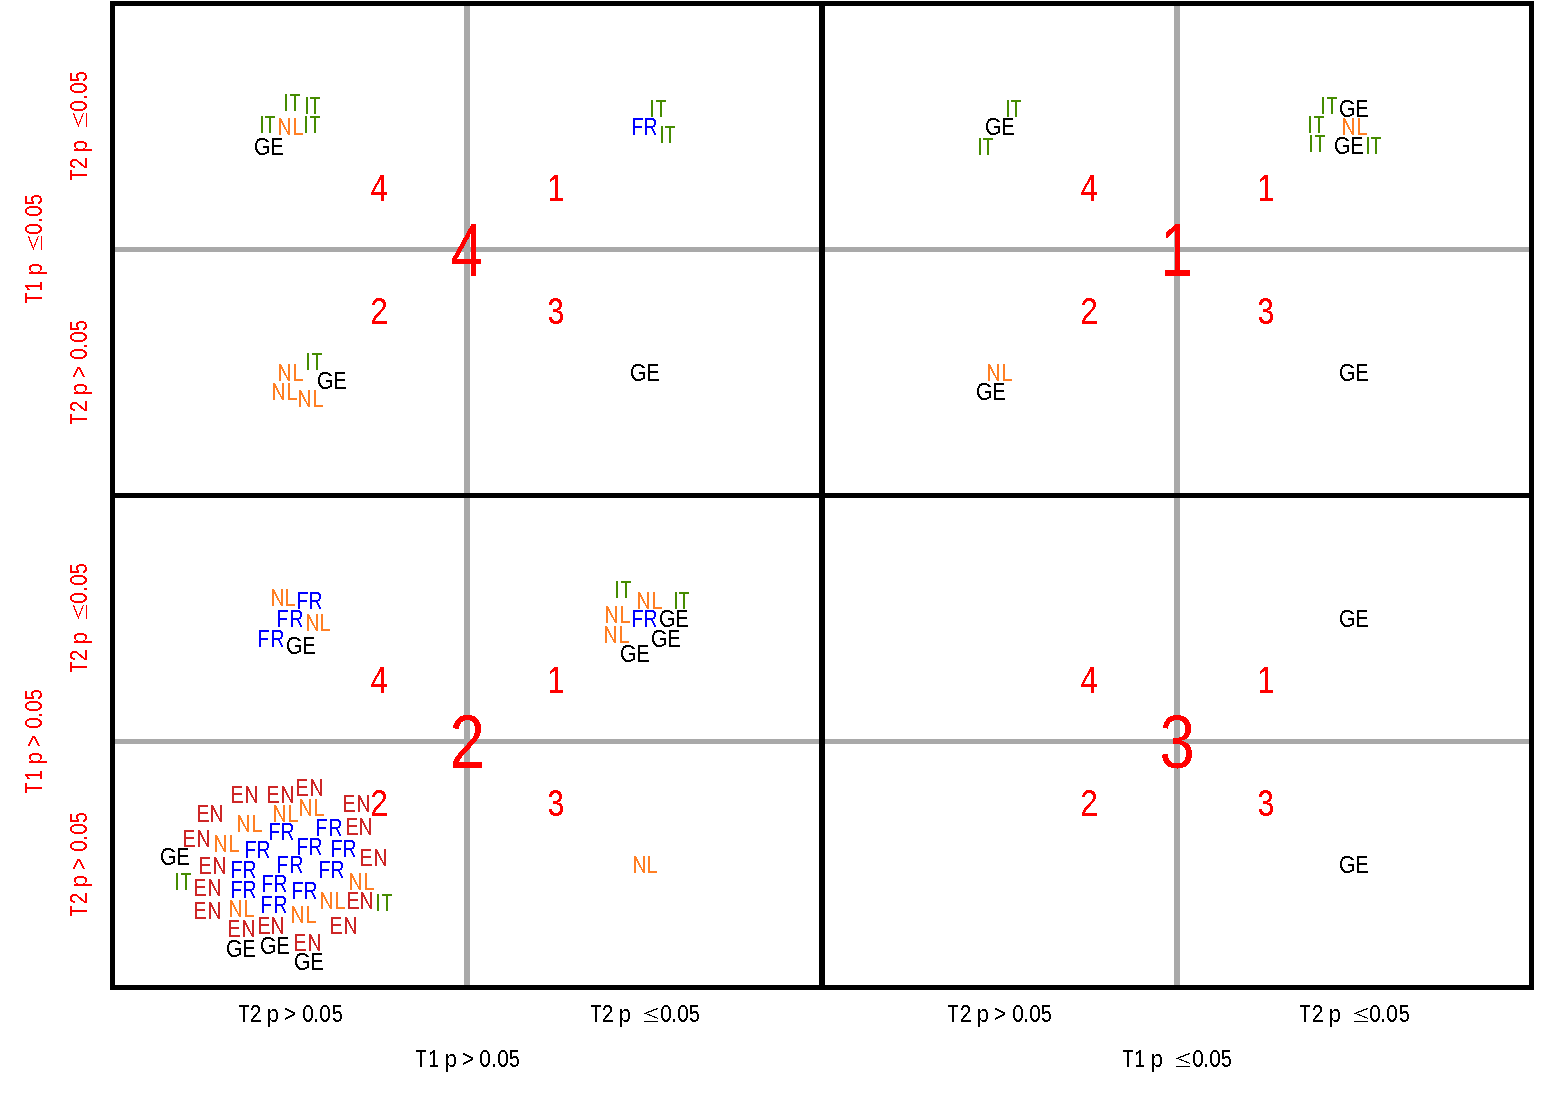
\includegraphics[width=\textwidth]{figures/04-5.pdf}
    \caption{EI task, [e] targets, individual processing strategies}
    \label{fig:04:5}
\end{figure}

The graph can be used to place SO and OS word orders in a hierarchy. At both test times, squares 1 and 2 represent extreme cases: square 1 contains learners who process both types of targets with above chance level accuracy; square 2 those who perform at or below chance level. Among the latter, 9 improved on both types of targets at T2 (scenario 2:1), while 6 showed an improvement on SO targets alone (scenario 2:4). A single participant improved on OS, but not SO targets (scenario 2:3). Scenario 1:1 indicates that all targets were processed with above-chance accuracy at both T1 and T2; scenarios 1:2, 1:3 and 1:4 indicates that performance was above chance at T1, but not so at T2, in which either SO (1:3), OS (1:4) or both types of targets (1:2) did not satisfy the criterion.

Squares 3 and 4 indicate a difference in the processing of word order. It is not unexpected that square 3, in which learners behave above chance on OS, but not SO targets, only comprises 2 learners at T1. The opposite scenario, square 4, comprises 15 learners at T1. 

Overall, it seems that if one value of word order is easier to process, or improves earlier than the other one, then in most cases it is SO. Nevertheless, the vast majority of participants at T1 is found in square 2, indicating chance-level behaviour on both target types.

The graph can also be used to study the evolution of processing strategies in the repetition task over time, depending on the word order of the target sentence. The first obvious observation is that for most learners, there is no evolution whatsoever. The bulk of the data set (42 learners out of 88) can be found in scenario 2:2, which indicates chance behaviour under all conditions (OS and SO targets, at both T1 and T2). This group includes all English L1 learners, most French, about a half of the Dutch, and only a few Italians and Germans. Conversely, 7 learners can be found in scenario 1:1, which indicates the presence of a morpho-syntactic processing strategy all the way from T1 to T2 on both OS and SO targets. Finally, the 6 learners in scenario 4:4 were able to process SO, but not OS targets at T1 and T2 alike.

A few learners show an improvement from T1 to T2. Some change towards more target-like processing strategies: this is the case of scenarios 2:4, 2:3 and 2:1, in which one finds learners who at T1 failed to systematically repeat [e] under any circumstances, but at T2 improved on SO, OS, or both target types, respectively. 

A few participants seem to move away from the target variety: learners in scenario 4:2 processed SO targets above chance at T1, but no longer do so at T2. Other surprising, though rare cases can be found in scenarios 1:3, 1:4 and 1:2: these learners were able to process all targets at T1, but at T2 failed to systematically repeat [e] in SO, OS and all targets, respectively. There might be various explanations for this rare and apparently illogical behaviour. In addition to variables beyond experimental control, such as motivation, tiredness, distractedness, equipment malfunction, such behaviour may be due to border-line scores at T1: even a single additional error thus could have determined their being on either side of the threshold. 

\subsection{Repetition of -[a]}\label{sec:04:2.5}

The data set concerning the repetition of [a] is characterised by an evident ceiling effects for all language groups (\figref{fig:04:6} and \tabref{tab:04:7}).

\begin{figure}
    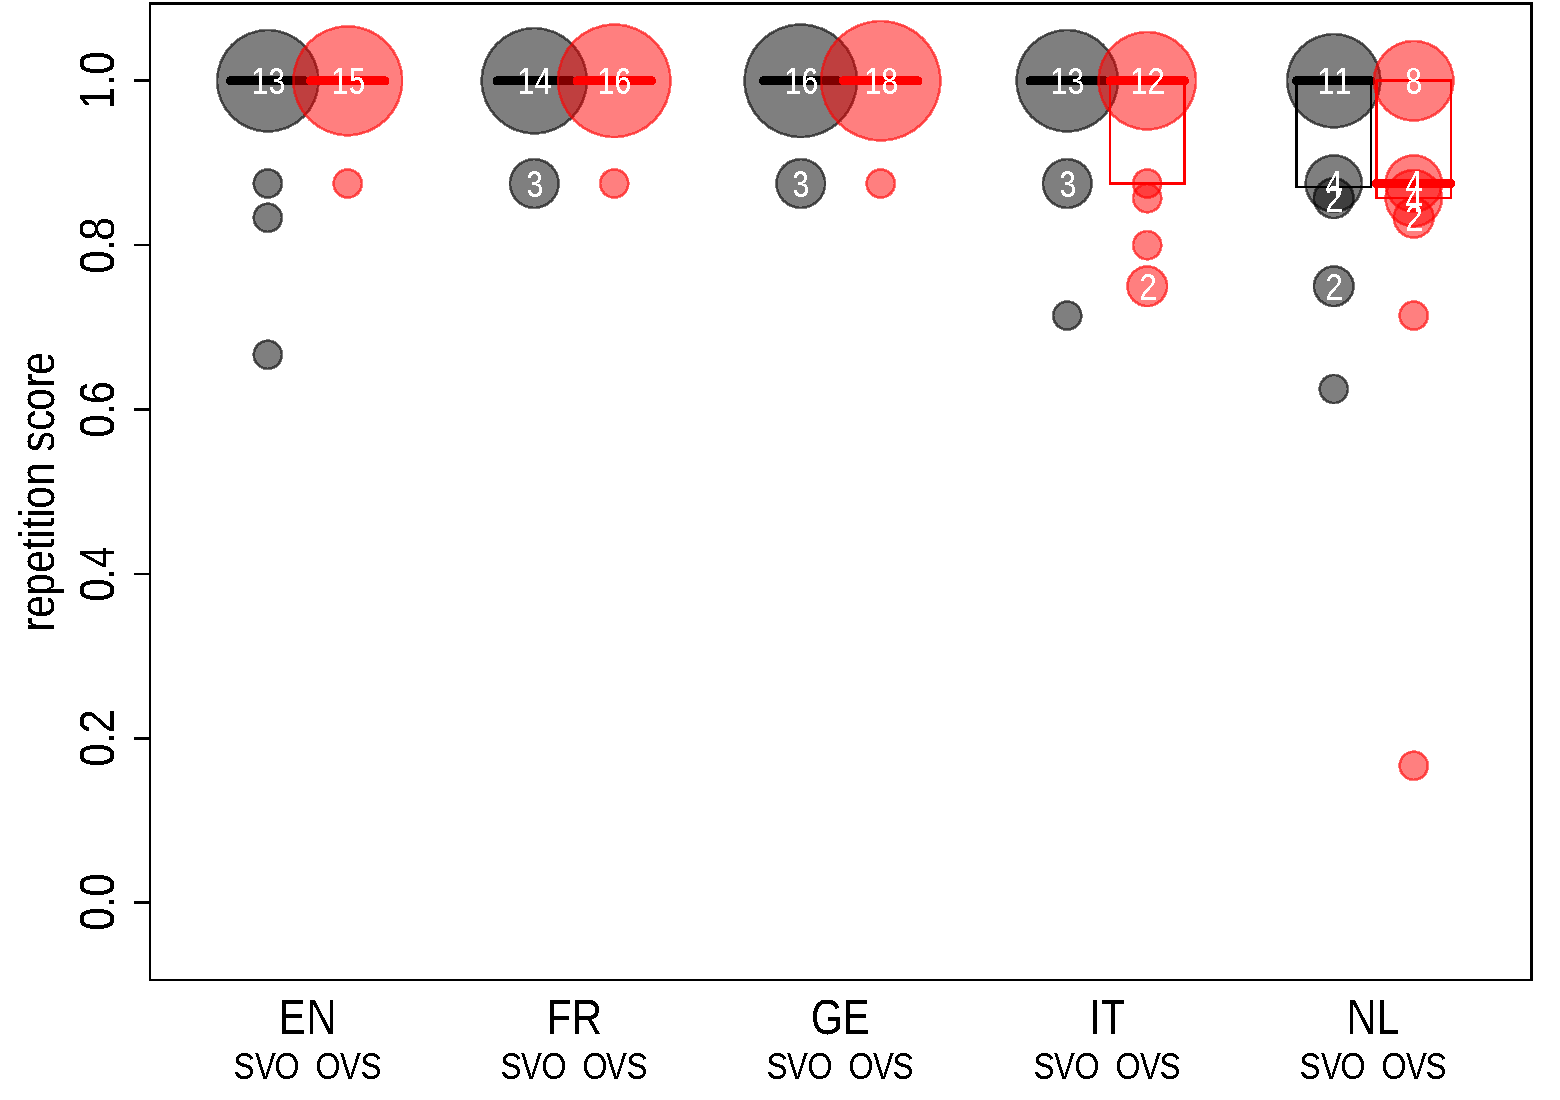
\includegraphics[width=\textwidth]{figures/04-6.pdf}
    \caption{EI task, [a] targets, T1, scores by L1}
    \label{fig:04:6}
\end{figure}

\begin{table}
    \begin{tabularx}{\textwidth}{XXXXXXr}
    \lsptoprule
    & &{SO}& & &{OS}&\\
    L1 & mean & sd & n & mean & sd & n\\
    \midrule
    FR & 0.98 & 0.15 & 127 & 0.99 & 0.09 & 130\\
    GE & 0.98 & 0.14 & 145 & 0.99 & 0.08 & 141\\
    IT & 0.96 & 0.19 & 133 & 0.95 & 0.23 & 128\\
    NL & 0.92 & 0.28 & 154 & 0.88 & 0.32 & 145\\
    EN & 0.96 & 0.20 & 101 & 0.99 & 0.09 & 116\\
    \lspbottomrule
    \end{tabularx}
    \caption{L1 group scores for the repetition of [a], T1}
    \label{tab:04:7}
\end{table}

As detailed in \chapref{sec:3}, in the VILLA input nominative [a] is indeed the most frequent and widespread ending in the paradigm of feminine nouns, in addition to instantiating both the citation form of lexical item as well as the form in which they were first introduced in the input. It is thus hardly surprising that it may overextend onto the much rarer and specialised accusative ending [e]. However, it is interesting to observe that some learners failed to repeat -[a] in all of the cases in which it was required; this tendency also seems to slightly vary across L1s. Since any output different from either [a] or [e] was excluded from the analysis, a failure to repeat [a] necessarily means that the marked ending [e] was produced. It is important to point out that this observation is not equivalent to saying that the accuracy of the repetition of [e] increases: the obligatory occurrences of [a] and [e] constitute different data-sets and are fully independent of each other. An error in the repetition of [a] may result in the two target sentence nouns being marked as [e], or alternatively to the swapping of the expected case endings, if an error is made in the repetition of target [e], too.

Curiously enough, the errors in the repetition of [a] seem to be maintained and even increase in number at T2 (\figref{fig:04:7} and \tabref{tab:04:8}).

\begin{figure}
    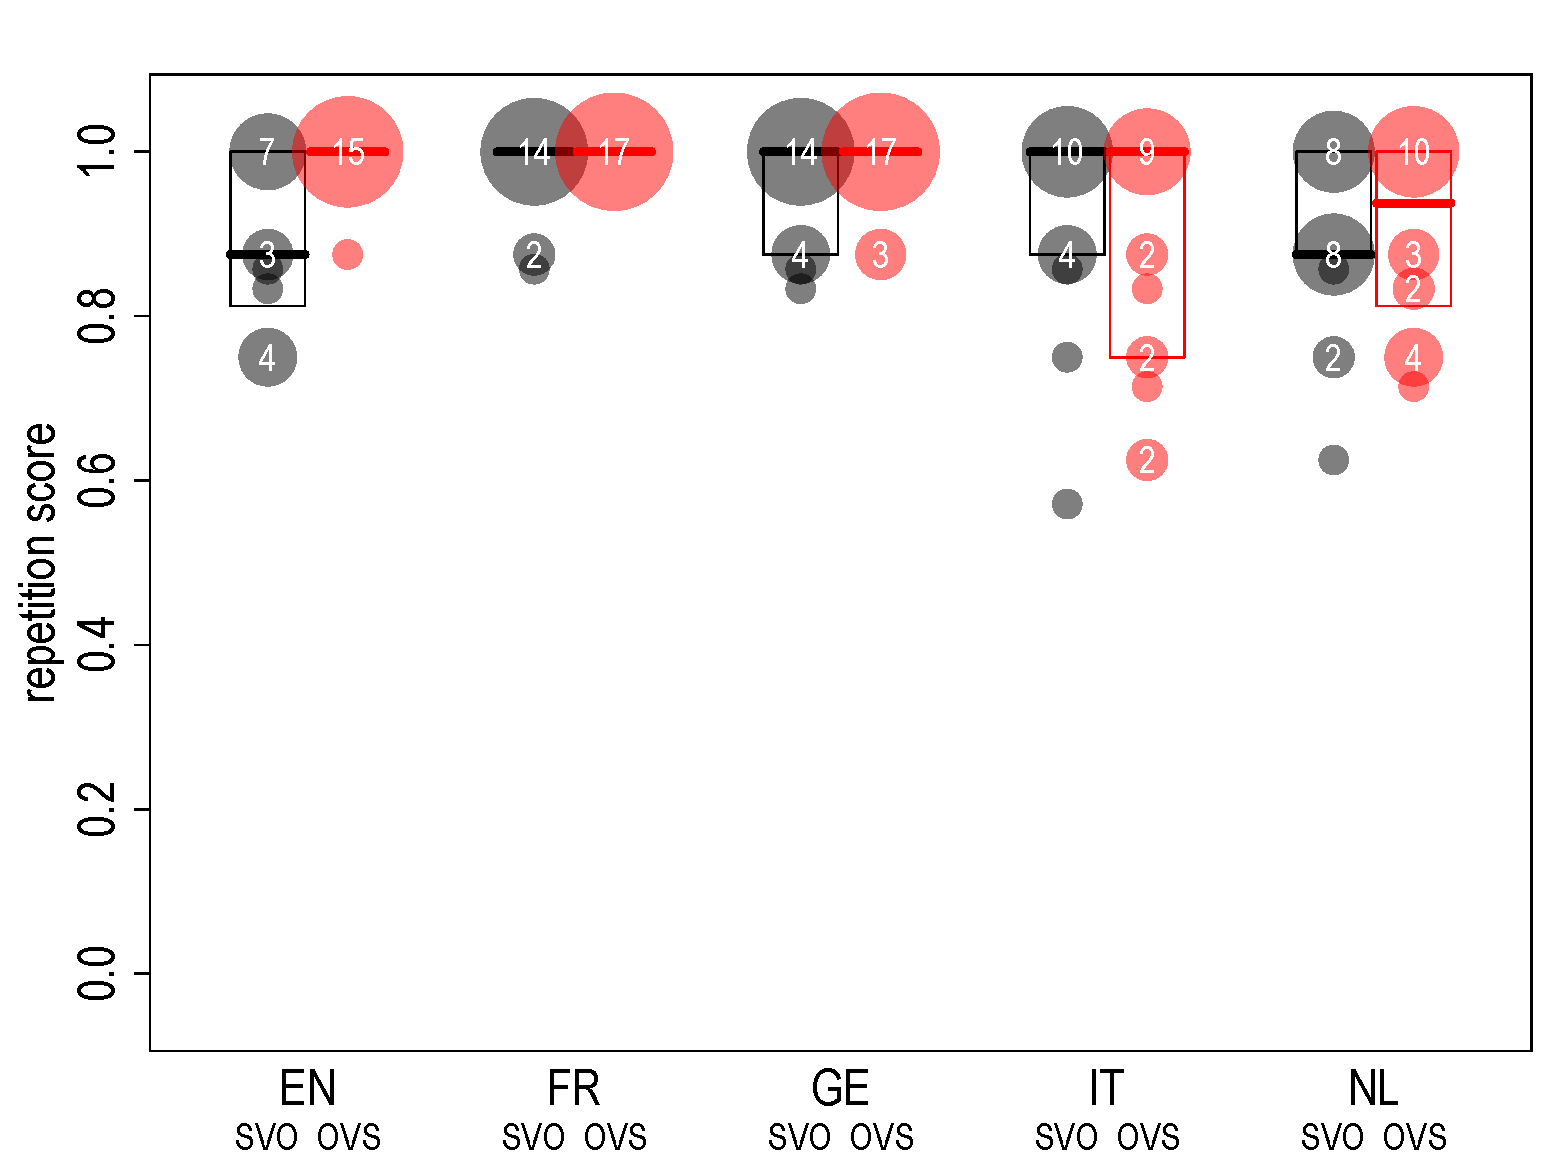
\includegraphics[width=\textwidth]{figures/04-7.pdf}
    \caption{EI task, [a] targets, T2, scores by L1}
    \label{fig:04:7}
\end{figure}

\begin{table}
    \begin{tabularx}{\textwidth}{XXXXXXr}
    \lsptoprule
    &  & {SVO} && & {OVS} &\\
    L1 & Mean & Sd & n & Mean & Sd & n\\
    \midrule
    FR & 0.98 & 0.15 & 132 & 1.00 & 0.00 & 133\\
    GE & 0.96 & 0.19 & 155 & 0.98 & 0.14 & 155\\
    IT & 0.93 & 0.26 & 134 & 0.88 & 0.32 & 128\\
    NL & 0.90 & 0.30 & 158 & 0.90 & 0.30 & 150\\
    EN & 0.89 & 0.31 & 119 & 0.99 & 0.09 & 119\\
    \lspbottomrule
    \end{tabularx}
    \caption{L1 group scores for the repetition of [a], T2}
    \label{tab:04:8}
\end{table}

\tabref{tab:04:9} lists the learners whose probability of correctly repeating -[a] does not differ from chance, again computed for each test time based on a binomial distribution described by the number of correct responses, the number of trials, and a 0.5 chance threshold. These learners do not appear to correctly repeat target [a] with a frequency which could be called systematic; the results are compatible with a strategy of guessing.

The table describes each observation in terms of participants, L1, word order and time: for each relevant combination it provides the number of correct responses, the number of trials and the resulting mean accuracy. Finally, the column “EI\_p” indicates the probability that the learner performed the task by guessing. As discussed in the previous section, this information should be discarded in the extreme cases in which all responses are either correct or incorrect, a scenario whose linguistic interpretation is quite clear anyway. These values are provided for both endings, with the following rationale: if the learner was truly guessing, then one should observe a chance result for both [a] and [e] targets, as these are the only two alternative answers between which one can chose.

\begin{table}
    \fittable{
    \begin{tabular}{l l l ll rr rr rr rr}
    \lsptoprule
    &  &  &  & \multicolumn{2}{c}{EI\_correct} & \multicolumn{3}{c}{EI\_trials} & \multicolumn{2}{c}{ EI\_mean} & \multicolumn{2}{c}{ EI\_p}\\
     Participant & L1 & WO & Time & {}-[a] & \multicolumn{2}{c}{ {}-[e]} & {}-[a] & {}-[e] & {}-[a] & {}-[e] & {}-[a] & {}-[e]\\
     \midrule
     2101 & NL & SO & 2 & 5 & \multicolumn{2}{c}{ 1} & 8 & 7 & 0.63 & 0.14 & 0.14 & 0.94\\
     2102 & NL & OS & 2 & 5 & \multicolumn{2}{c}{ 0} & 7 & 8 & 0.71 & 0.00 & 0.06 & 1.00\\
     2104 & NL & OS & 1 & 1 & \multicolumn{2}{c}{ 2} & 6 & 8 & 0.17 & 0.25 & 0.89 & 0.86\\
     2108 & NL & SO & 1 & 5 & \multicolumn{2}{c}{ 8} & 8 & 8 & 0.63 & 1.00 & 0.14 & 0\\
     2118 & NL & OS & 1 & 5 & \multicolumn{2}{c}{ 3} & 7 & 6 & 0.71 & 0.50 & 0.06 & 0.34\\
     3119 & EN & SO & 1 & 4 & \multicolumn{2}{c}{ 0} & 6 & 7 & 0.67 & 0.00 & 0.11 & 1\\
     5105 & IT & SO & 1 & 5 & \multicolumn{2}{c}{ 7} & 7 & 8 & 0.71 & 0.88 & 0.06 & <.00\\
     5105 & IT & SO & 2 & 4 & \multicolumn{2}{c}{ 7} & 7 & 7 & 0.57 & 1.00 & 0.23 & 0\\
     5106 & IT & OS & 2 & 5 & \multicolumn{2}{c}{ 4} & 7 & 8 & 0.71 & 0.50 & 0.06 & 0.36\\
     5114 & IT & OS & 2 & 5 & \multicolumn{2}{c}{ 3} & 8 & 6 & 0.63 & 0.50 & 0.14 & 0.34\\
     5115 & IT & OS & 2 & 5 & \multicolumn{2}{c}{ 6} & 8 & 8 & 0.63 & 0.75 & 0.14 & 0.04\\
    \lspbottomrule
    \end{tabular}
    }
    \caption{EI task, repetition of –[a] at chance level}
    \label{tab:04:9}
\end{table}

A few comments can be made. First, these learners belong to only three L1 groups, the vast majority being speakers of Dutch or Italian. 5105 appears in the table twice because data were collected at both at T1 and T2. Word order and test time, in contrast, are fairly varied. 

Some learners (2108, 2118, 5105 at T2, 5115) seem to perform better on the repetition of [a]  than of [e]. All other learners conform to the expected pattern, in which repeating [a] appears somewhat easier than repeating [e]. As far as the ending [a] is concerned, the repetition score of some of the participants (2102, 2118, 5105 at T1, 5106) only slightly fails to reach statistical significance: typically, their p value  is 0.06, their mean 0.71, and the correct/total ratio is 5/7, which means that they made two errors out of seven trials. All appear to have missed a trial, which in turn may mean that they supplied an ending other than -[a] or -[e], or alternatively that they failed to repeat an entire target stimulus. In the former case, this behaviour may witness to a certain creativity on their side, which is an indication of system restructuring. The latter case may be speculatively linked to the fact that some participants spent a long time on the distracting phase of the exercise (copying a geometric figure on the answer sheet), which may have somewhat confused their memory of the target. In any case, the 0.05 threshold was set arbitrarily with the purpose of indicating a reasonably small probability, and one could argue that 0.06, although undoubtedly greater, is not so much greater.

These findings may be seen against the bigger picture of -[a] processing. Based on the rationale introduced in the preceding section, \figref{fig:04:8} plots learners according to their performance on the repetition of [a] in OS (horizontal axis, black) and SO (vertical axis, red) targets at T1 and T2.

\begin{figure}
    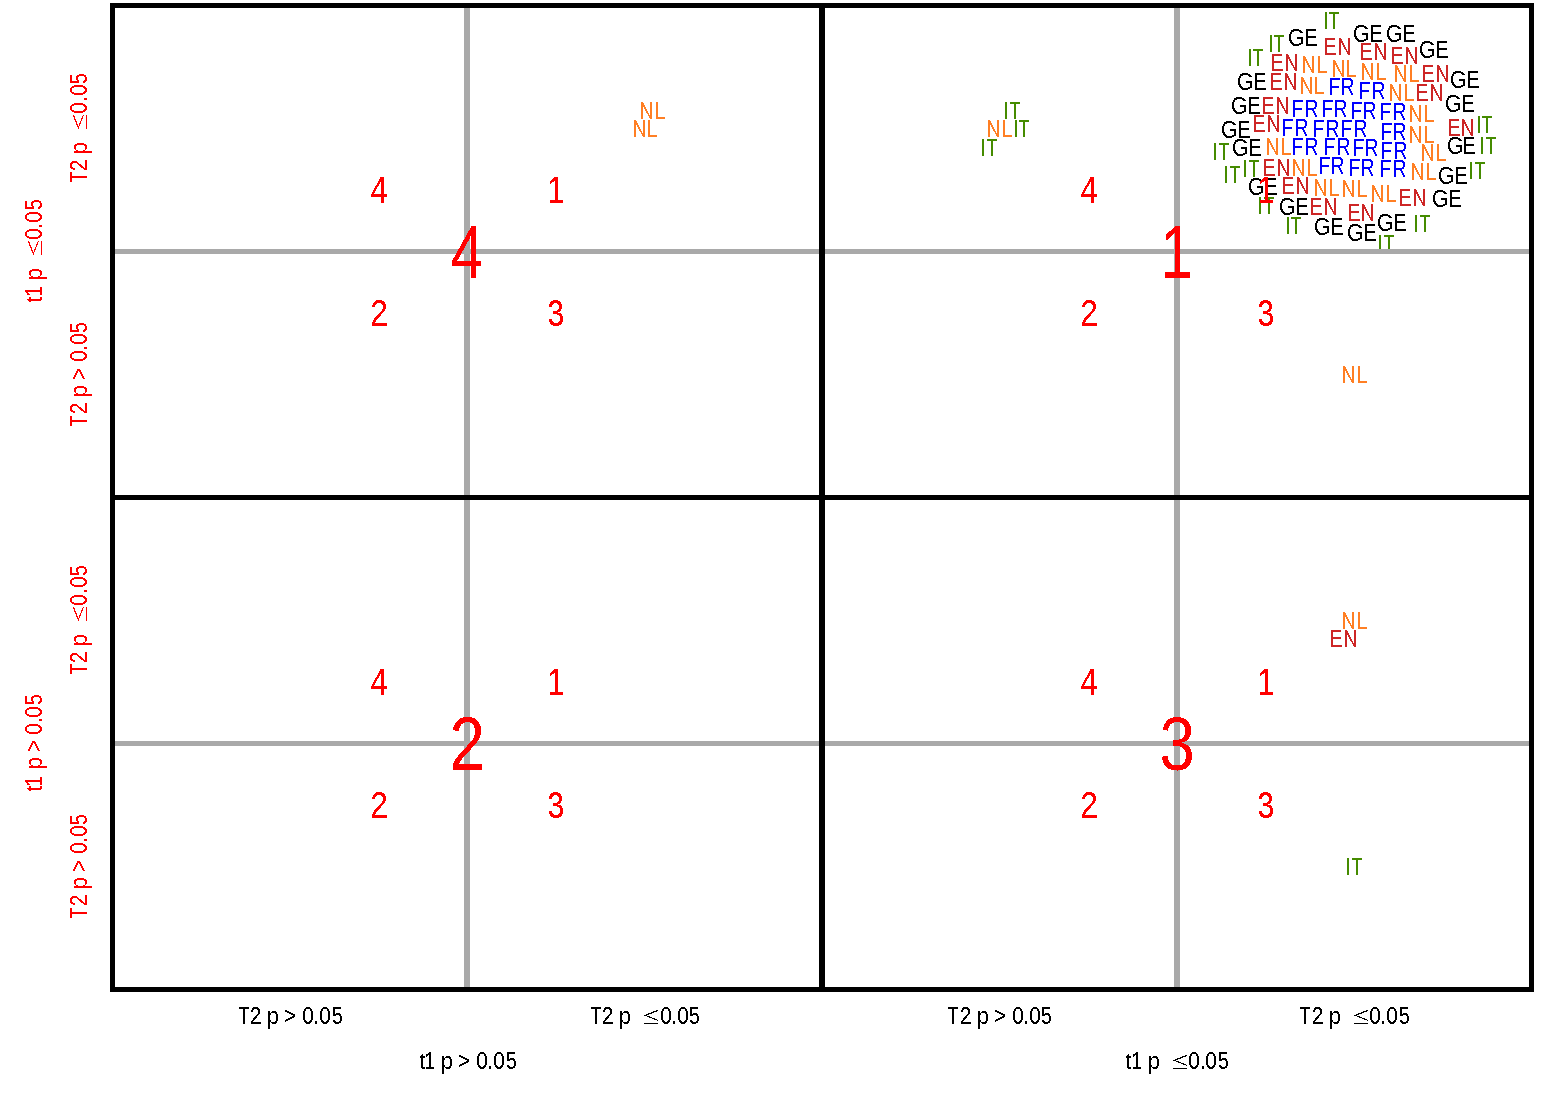
\includegraphics[width=\textwidth]{figures/04-8.pdf}
    \caption{EI task, [a] targets, individual processing strategies}
    \label{fig:04:8}
\end{figure}

Virtually all learners lie in scenario 1:1, which corresponds to scores above chance on OS and SO targets alike at both T1 and T2. The few data-points in other scenarios correspond to the 10 learners just discussed.

\section{Summary}\label{sec:04:3}

The VILLA EI test highlighted several tendencies, which may be summarised as follows:

\begin{itemize}
    \item Morphological marking, i.e. the presence of the non-basic case ending [e] is apparently more widespread in SO than OS targets.
    \item There is a clear effect of cross-linguistic influence in the case of the groups with the highest (L1 German) and lowest (L1 English) scores. The performance of the Italian group is also in line with that of the German participants, although this result was not expected based on contrastive analysis.
    \item Further exposure to the input is clearly beneficial to the development of morpho-syntactic skills.
\end{itemize}

It should be borne in mind that in the absence of a comprehension or a translation task it is impossible to verify what learners really meant to say (if anything) through their output. This in turn raises doubts as to the layer of language effectively targeted by the task: in the absence of this information, it is quite possible that learners did not reproduce the content of the stimulus sentence based on their provisional interlanguage grammar, as assumed by the rationale of the task, but simply repeated it as a string of sounds. Both hypotheses have supporting evidence. The rote repetition hypotheses seems realistic in light of output in which target lexical items are hardly recognisable, which suggests that the learner was not striving to reproduce them based on a mental representation, however approximate, but simply tried to retrieve them as sounds from working memory.

On the other hand, the notable difference between the repetition accuracy of the [e] ending in SO as opposed to OS targets suggest that there may be an effect of syntactic structure, which of course can only be hypothesised if the learner processes targets for meaning and attempts to identify their grammatical structure. Even in this case, however, an alternative perception-based explanation may be proposed: in SO targets, the non-basic [e] ending is found in the maximally salient word-final position, which may facilitate its being noticed and reproduced by learners even in the absence of processing for meaning.

In sum, it seems that while a few clear tendencies may be identified, based on the EI data alone it is impossible to definitively establish whether learners' output is based on morphosyntactic processing or perceptual prominence. In order to better describe the behaviour of the VILLA learners the following two chapters will make use of a comprehension test, whose results will prove useful to interpret the output of the EI task.
